\chapter{問題設定}
\label{chap:settings}

第\ref{chap:settings}章では,まず本研究で扱うデータセットについて説明し,続いて問題設定について述べる.

\section{データセット}

本研究では,映像予測の研究分野で一般的に用いられるBAIR Push Dataset\cite{ebert2017selfsupervised}を用いて各手法を評価する.データセットの模式図を図(\ref{fig:dataset})に示す.BAIR Push Datasetは行動条件付き映像予測と行動条件をつけない映像予測のどちらの研究でも用いられるデータセットであり,カリフォルニア大学バークレー校によって制作・公開されている.
このデータセットは,雑多な物体がおかれた机の上をロボットアームがランダムに掻き乱すようにして様々なデータが記録されており,今回はその中から行動系列$\vec{a}$と固定視点から観測された画像系列$\vec{o}$を用いる.今回用いる行動系列$\vec{a}$は,具体的にはロボットのエンドエフェクタの位置姿勢の命令値で,4次元のベクトルになっている.観測画像は64x64サイズのRGB画像で,これらのデータは10hzで撮られている.また訓練時と評価時に使われる物体は揃えられている.


\section{問題設定}

本研究では行動条件付き映像予測の問題を解く.問題設定の模式図を図(\ref{fig:settings})に示す.具体的には,初期観測$o_0$とある行動主体が実行した行動系列$a_{1:10}$が与えられたときに$o_{1:10}$を生成し,その生成される映像の尤度を高めることを目指す.ただし訓練時には行動系列と観測系列の組$\{\vec{a}, \vec{o}\}$の訓練用のデータセットを用いることができ,評価時には,訓練データには含まれないが訓練データと同じ条件で収集された評価用のデータセットを用いる.
本研究の目的は,この行動条件付き映像予測問題においてベースラインにDSSMを設定し,DSSMをより複雑な環境での映像予測問題にもスケールできるように拡張することである.

\begin{figure}[h]
    \begin{center}
      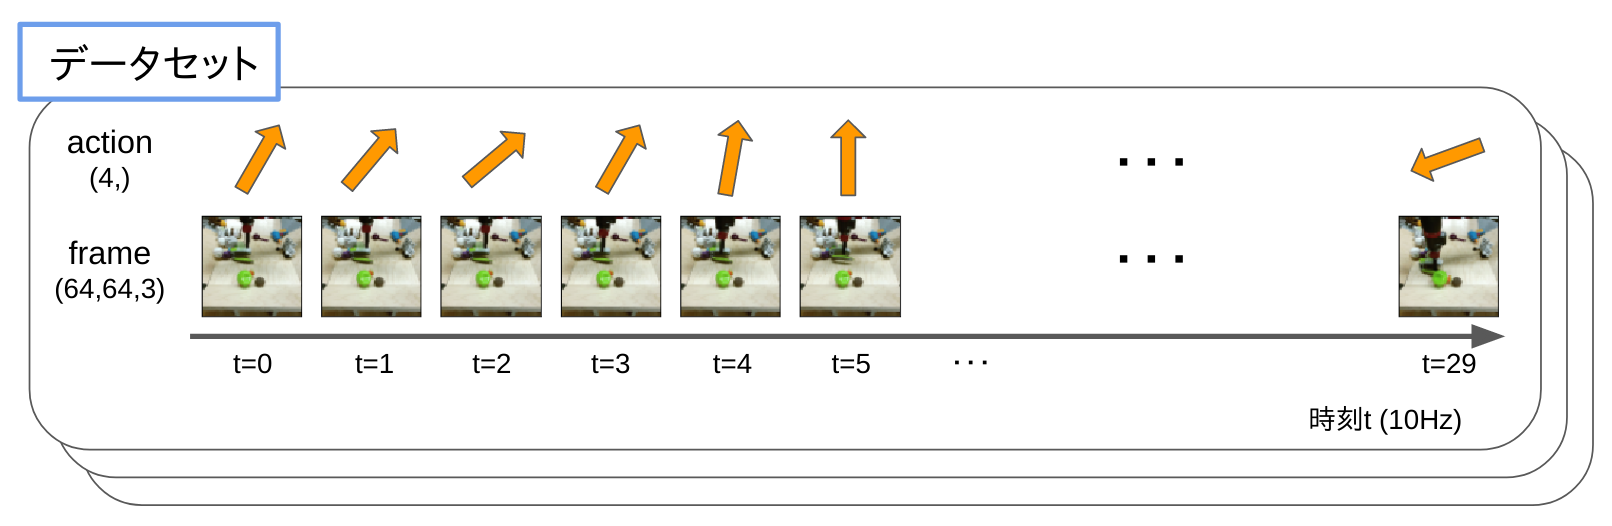
\includegraphics[scale=0.22]{./figures/dataset.png}
      \caption[データセットの模式図]{データセットの模式図.括弧内の数字はデータの次元を示す.}
      \label{fig:dataset}
    \end{center}
  \end{figure}

\begin{figure}[h]
\begin{center}
    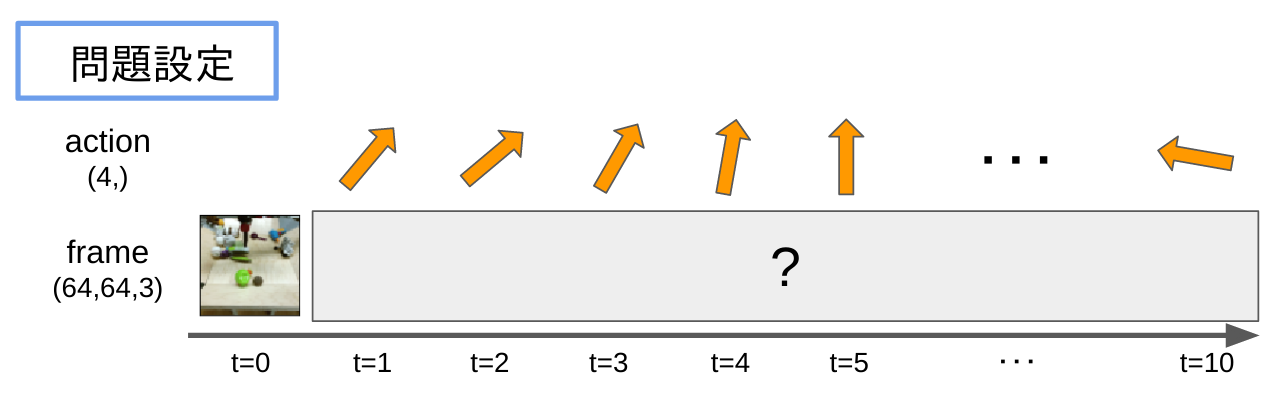
\includegraphics[scale=0.25]{./figures/settings.png}
    \caption[問題設定の模式図]{問題設定の模式図.初期観測と行動系列が与えられたときに将来の観測を生成する.}
    \label{fig:settings}
\end{center}
\end{figure}